\section{Subsistema: Mecânica e Alimentação}

  \subsection{Sistema de Tração}

  Para a análise comparativa foram estudadas e consideradas as características dos principais tipo de sistemas de tração,
  afim de escolher um sistema que atenderá todas as necessidades do projeto sendo o menos oneroso.

  \begin{itemize}
    \item Sistema de Esteira

    O sistema de tração por esteiras é largamente utilizado em aplicações agrícolas e em aplicações gerais nas quais é necessária
    a locomoção em terreno acidentado. O sistema tradicional de transmissão mecânica por esteiras é formado por diversos componentes,
    como conversor de torque, amortecedores e \textit{dumpers}.
    Este sistema possui como vantagem o alto fornecimento de tração ao veículo, mas requer um grande espaço para acoplamento ao mesmo,
    além da baixa disponibilidade de materiais para sua fabricação. Outra desvantagem é que este sistema impede que o veículo realize
    manobras de contra-rotação.

    \item Sistema de Rodas

    O sistema de rodas consiste na configuração mais utilizada em todos os tipos de veículos, a literatura é bastante consolidada
    no que se refere a sistemas de transmissão e acoplamentos para veículos movidos sobre rodas. Este sistema foi o escolhido para
    implantação neste projeto devido à sua viabilidade de projeto e fabricação.
    Foi realizada uma pesquisa de modelos de rodas disponíveis, tendo como requisito um diâmetro de aproximadamente 10cm e pneus com
    perfil off-road, conforme mostra a figura \ref{WHEELS}.

    \begin{figure}[!htb]
    \begin{center}
    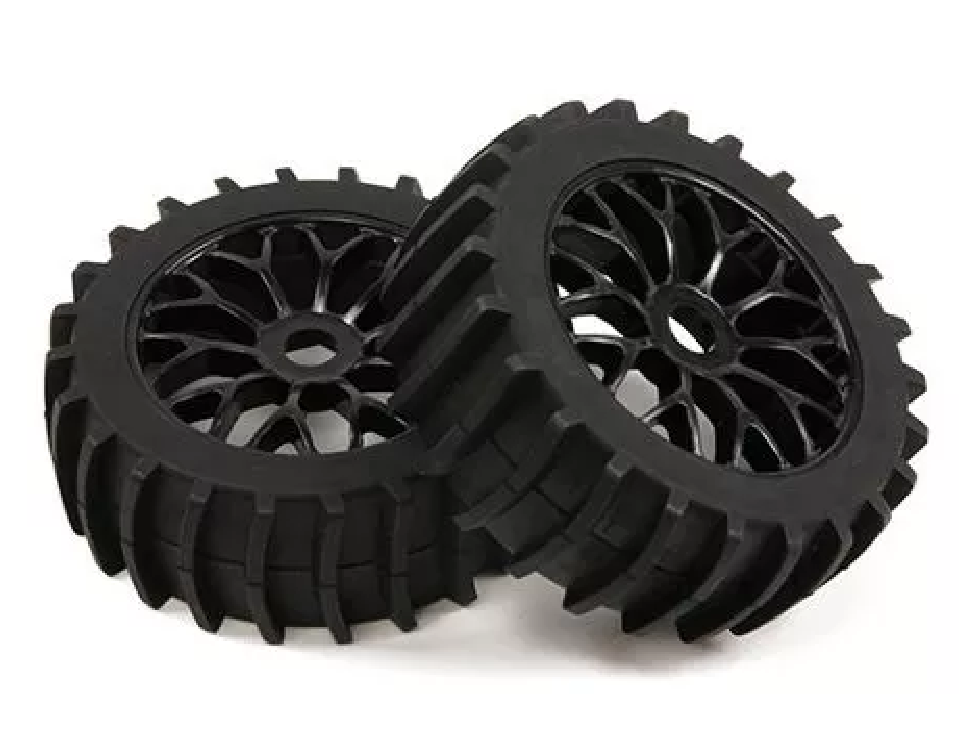
\includegraphics[keepaspectratio=true,scale=0.3]{figuras/wheels.eps}
    \caption{\label{WHEELS}Modelo de rodas}
    \end{center}
    \end{figure}

		\newpage
    \item Sistema Aranha

    Este sistema de locomoção é bastante engenhoso. Consiste em vários braços, geralmente 6 ou 8, comandados por 2 motores ou
    mais em cada braço. Este sistema pode ser usado nos mais diversos tipos de terreno por fornecer alta estabilidade e tração
    satisfatória. A cinemática envolvida na movimentação e no controle deste tipo de sistema é muito mais complexa do que nos
    sistemas de locomoção por esteira e por rodas, devido ao alto número de motores requeridos.

  \end{itemize}

  Dentre as outras alternativas, adotou-se a locomoção baseada em rodas, pois são mais comumente encontrados na robótica móvel,
  tendo em vista o baixo custo, seja na implementação como na manutenção, fornece uma boa estabilidade, além de sua simplicidade
  mecânica. Como será aplicado em terrenos planos com algumas irregularidades, sem grandes declives e aclives \cite{matsumura2014desenvolvimento}, portanto a alternativa
  atende bem a proposta.

  Foi escolhido rodas de diâmetro grande, pois com ela o sistema de tração fica mais simples e com custos menores. O veículo também poderá passar por pequenos obstáculos sem dificuldades. Com esse conjunto o robô ficará elevado em relação ao solo, levando em conta seu centro de gravidade e demais componentes atuando. A figura \ref{WHEEL} mostra o tipo de roda relatada.

  \begin{figure}[!htbp]
  \begin{center}
  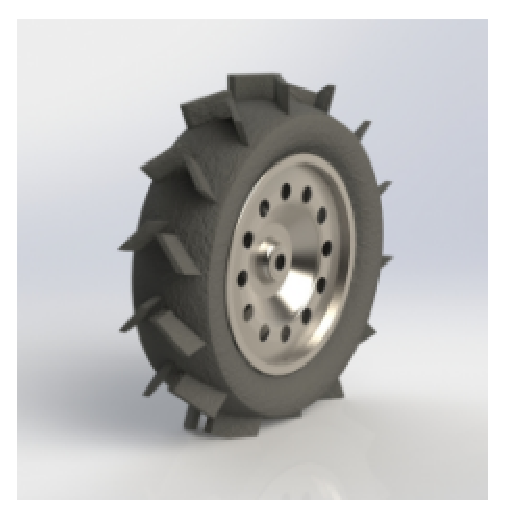
\includegraphics[keepaspectratio=true,scale=0.5]{figuras/wheel.eps}
  \caption{\label{WHEEL}Roda escolhida para o projeto}
  \end{center}
  \end{figure}

  \newpage
  \vfill
  \pagebreak

  \subsection{Sistema de Direção}
    O sistema de direção adotado será o de duas barras birrotuladas, onde uma delas será acoplada ao servomotor de direção por um conjunto de pinhão e cremalheira. O motor de direção para este sistema, deverá forncer um grau de liberdade de até 180º, devido a movimentção do veículo. No entanto o modelo a ser usado é o servo digital power Hd.

  \subsection{Sistema de Suspensão}
  Como o terreno estudado possui algumas irregularidades, é necessário amortecimento em cada uma das rodas do veículo, portanto é preciso a inserção de um sistema de suspensão independente para as rodas traseiras (geometria \textit{McPherson}) e dependente para o conjunto de rodas dianteiras (geometria de eixo rígidos/eixo de torção).

  Suspensões independentes garantem melhor estabilidade aos veículos, em detrimento de maior custo e complexidade de fabricação; neste caso usa-se este sistema no eixo traseiro devido a tração do veículo ser apenas neste eixo. Já as suspensões dependentes são mais fáceis de fabricar e instalar, porém fornecem menor estabilidade ao veículo.

  Nas figuras \ref{SUSPENTION01} e \ref{SUSPENTION02} estão alguns exemplos quanto ao sistema de transmissão e o tipo de roda escolhida.

  \vfill

  \begin{figure}[!htbp]
  	\begin{center}
  		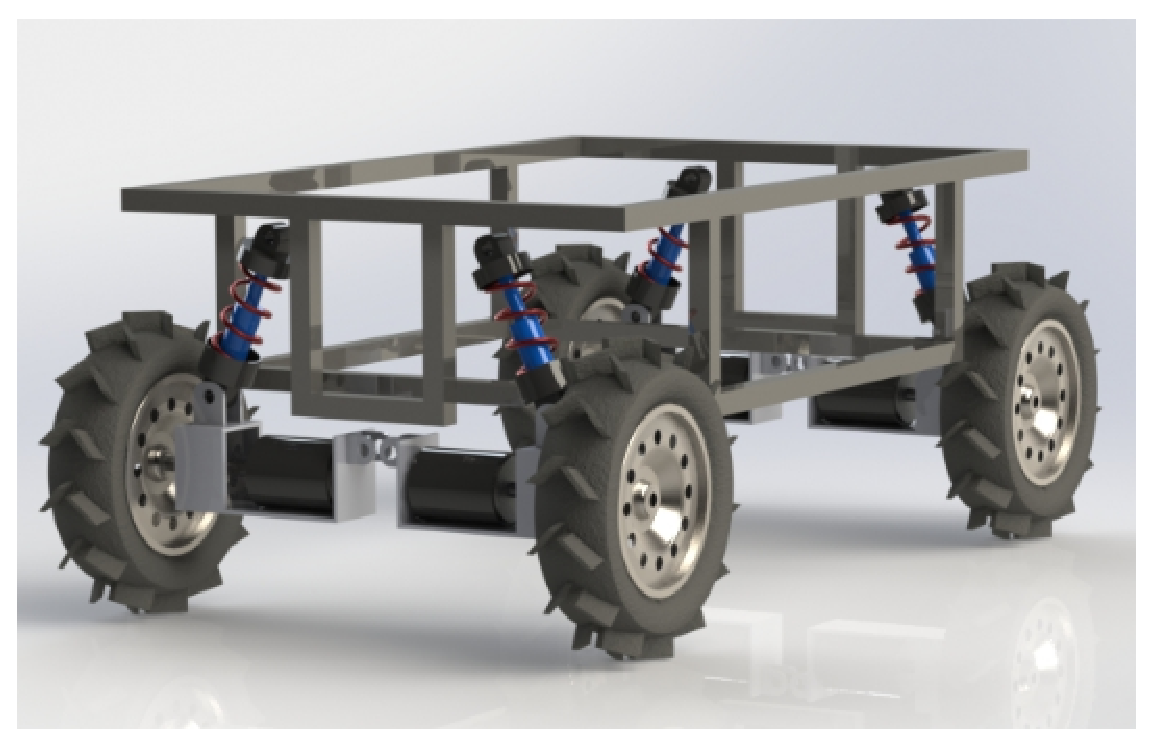
\includegraphics[keepaspectratio=true,scale=0.5]{figuras/suspention01.eps}
  		\caption{\label{SUSPENTION01}Roda, suspensão e chassi Renderizados}
  	\end{center}
  \end{figure}

  \begin{figure}[!htbp]
  	\begin{center}
  		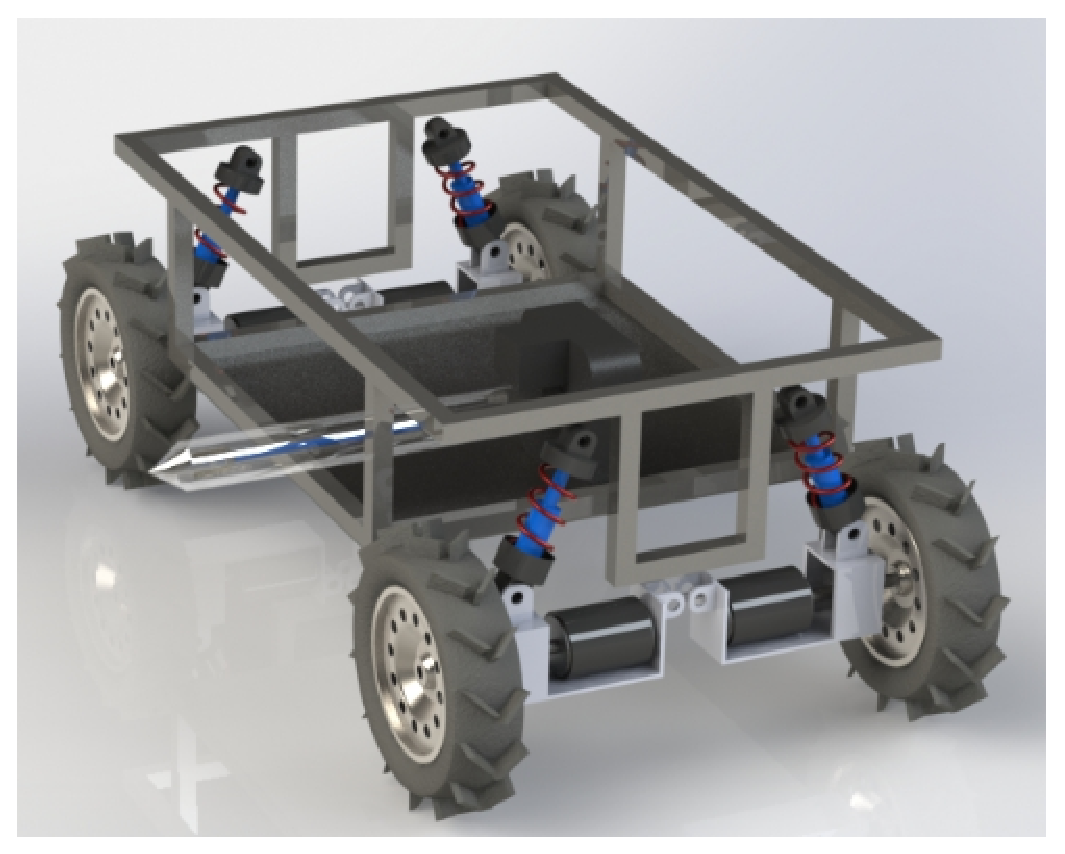
\includegraphics[keepaspectratio=true,scale=0.5]{figuras/suspention02.eps}
  		\caption{\label{SUSPENTION02}Roda, suspensão e chassi Renderizados}
  	\end{center}
  \end{figure}
  
    \begin{figure}[!htbp]
    	\begin{center}
    		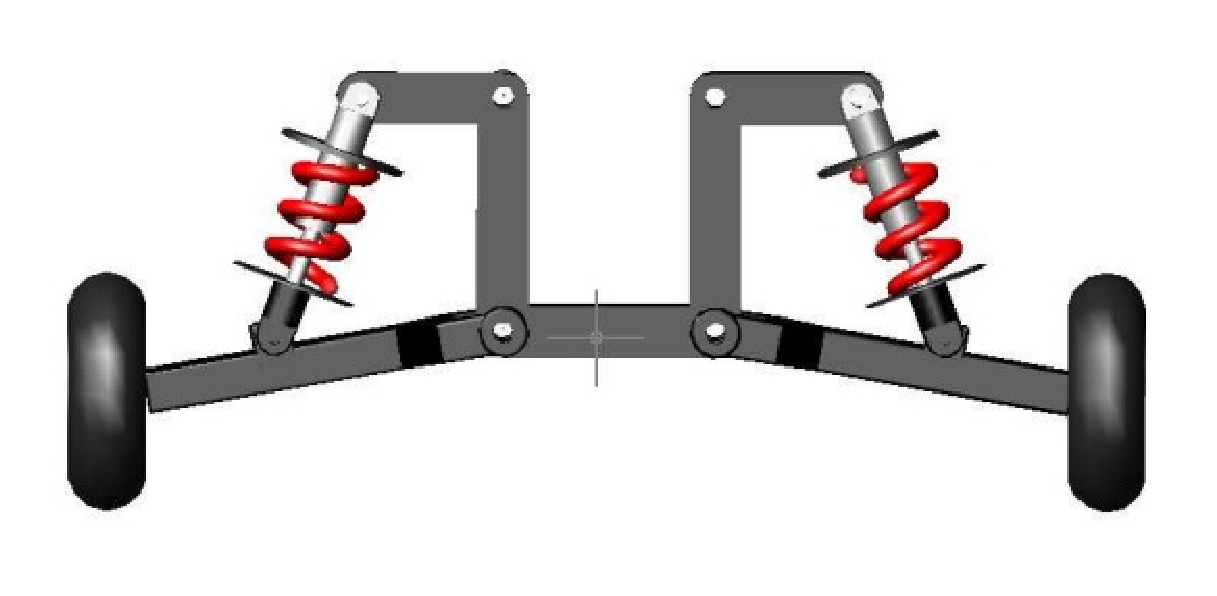
\includegraphics[keepaspectratio=true,scale=0.5]{figuras/sistema_de_suspencao.eps}
    		\caption{\label{sistema_suspencao}Sistema de suspenção}
    	\end{center}
    \end{figure}
    
      \begin{figure}[!htbp]
      	\begin{center}
      		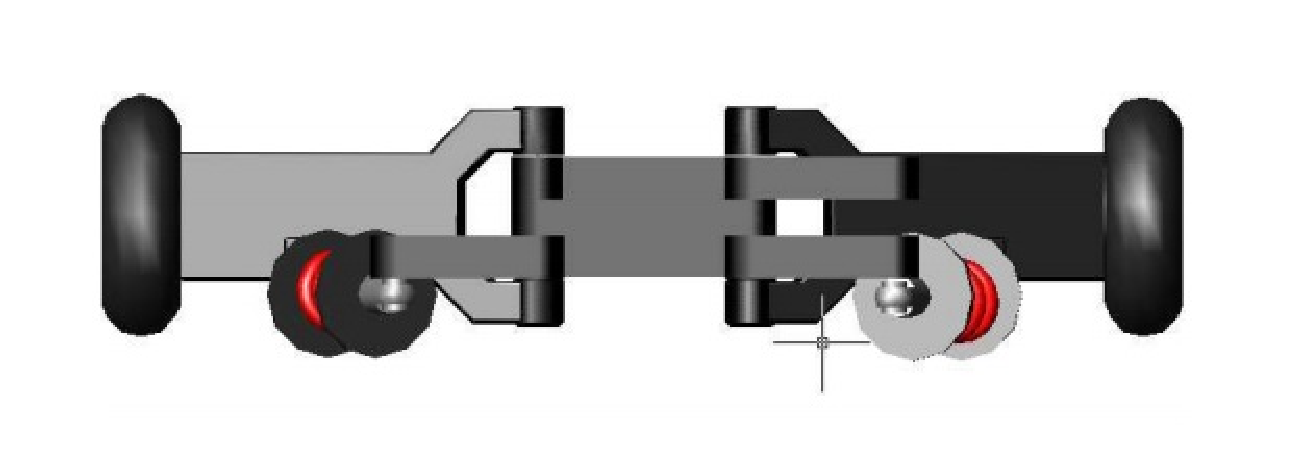
\includegraphics[keepaspectratio=true,scale=0.5]{figuras/sistema_de_suspencao_cima.eps}
      		\caption{\label{sistema_suspencao_cima}Sistema de suspenção vista de cima}
      	\end{center}
      \end{figure}
  
  \newpage
  
  \subsection{Estrutura}
  Após a definição dos sistemas que compõem a parte mecânica deste projeto é necessário a definição de uma estrutura externa para o veículo (rodas, pneus, chassi, eixos, carenagem e suspensão). Foi feita uma pesquisa para verificar quais materiais atenderiam as necessidades da estrutura do veículo. Portanto seguem as tabelas comparativas de possíveis materiais a serem usados.

  \begin{table}[!htbp]
  \begin{center}
  \caption{Roda e Pneu}
  \begin{tabular}{|p{2cm}|p{3cm}|p{2cm}|p{4cm}|}
  \hline
  \textbf{Roda e Pneu} & \textbf{Descrição} & \textbf{Imagem} & \textbf{Link}\\\hline\hline
  Tipo 1 & Roda de MBS Atom, 80/85 ou Colt 80 placas, de 7 polegadas & 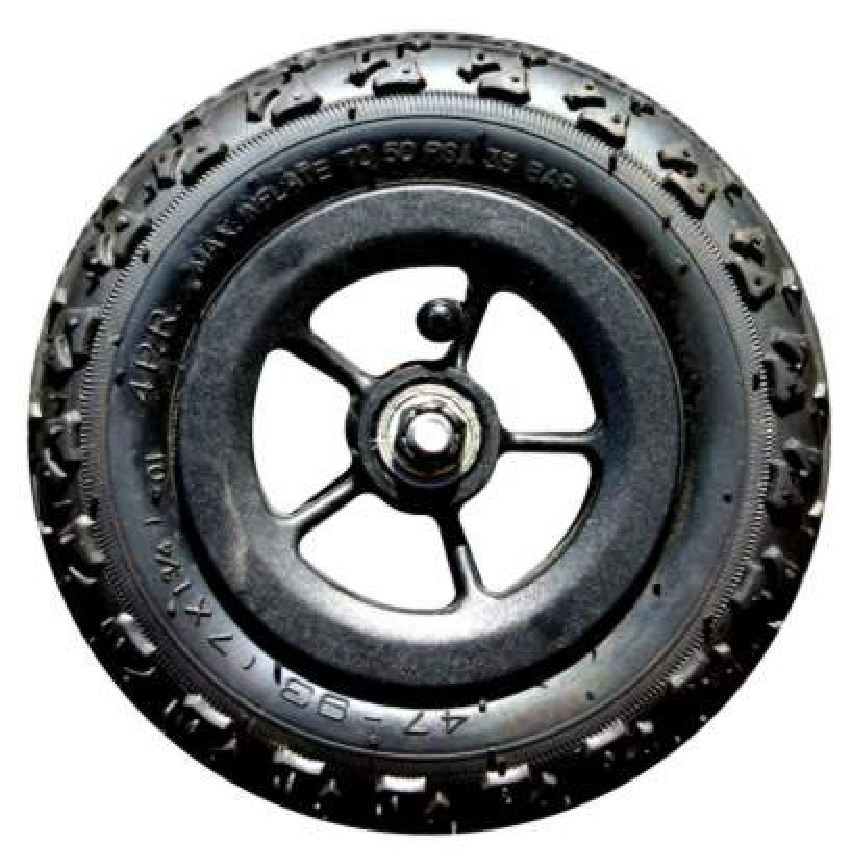
\includegraphics[width=2cm]{figuras/roda_mbs.eps} & \href{http://shop.mbs.com/accessories-488/mountainboard-wheels/complete-wheels/complete-7-wheel.html}{shop.mbs.com}\\\hline
  Tipo 2 & Rodas 17mm Buggy Off Road Pneu Para Areia E Terra -FH & 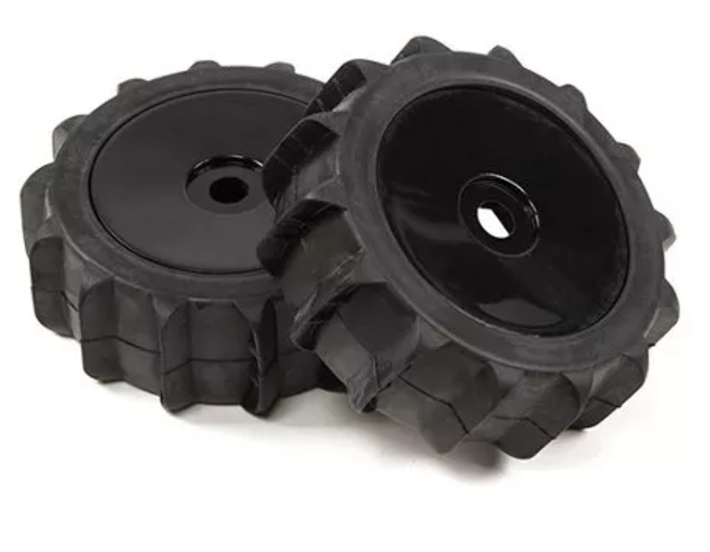
\includegraphics[width=2cm]{figuras/roda_buggy.eps} & \href{http://produto.mercadolivre.com.br/MLB-788601174-par-de-rodas-17mm-buggy-off-road-pneu-para-areia-e-terra-fh-_JM}{mercadolivre.com.br}\\\hline
  \end{tabular}
  \end{center}
  \end{table}

  \begin{table}[!htbp]
  \begin{center}
  \caption{Chassi}
  \begin{tabular}{|p{2cm}|p{3cm}|p{2cm}|p{4cm}|}
  \hline
  \textbf{Chassi} & \textbf{Material} & \textbf{Imagem} & \textbf{Link}\\\hline\hline
  Tipo 1 & Aço inox & 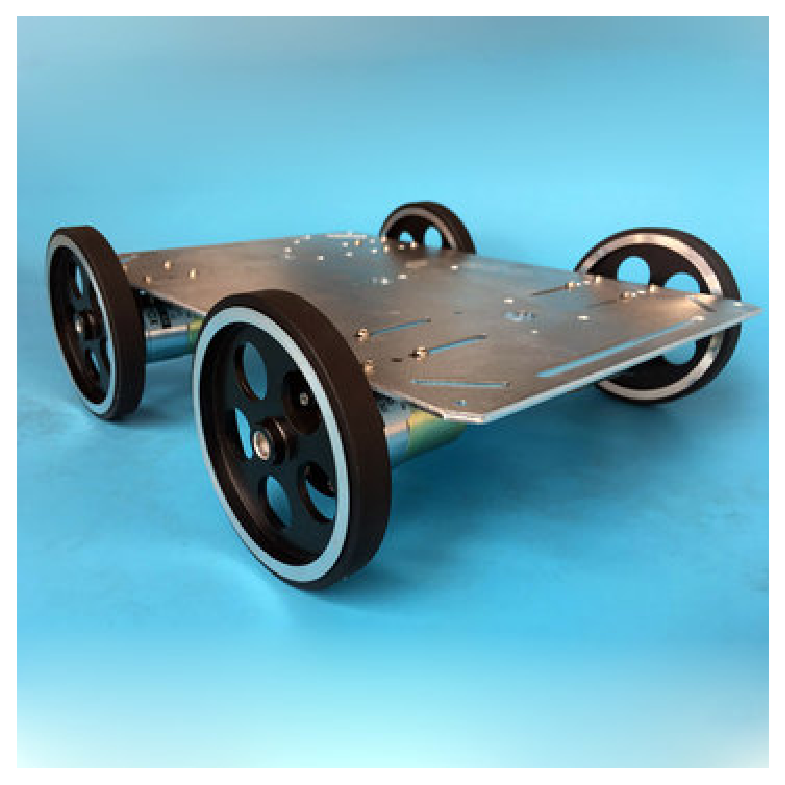
\includegraphics[width=2cm]{figuras/chassi_inox.eps} & \href{http://www.banggood.com/pt/DIY-C600-DIY-Remote-Control-Crawler-Chassis-Smart-Track-Stainless-Stell-Metal-Tank-p-1079216.html}{banggood.com}\\\hline
  Tipo 2 & Aluminio & 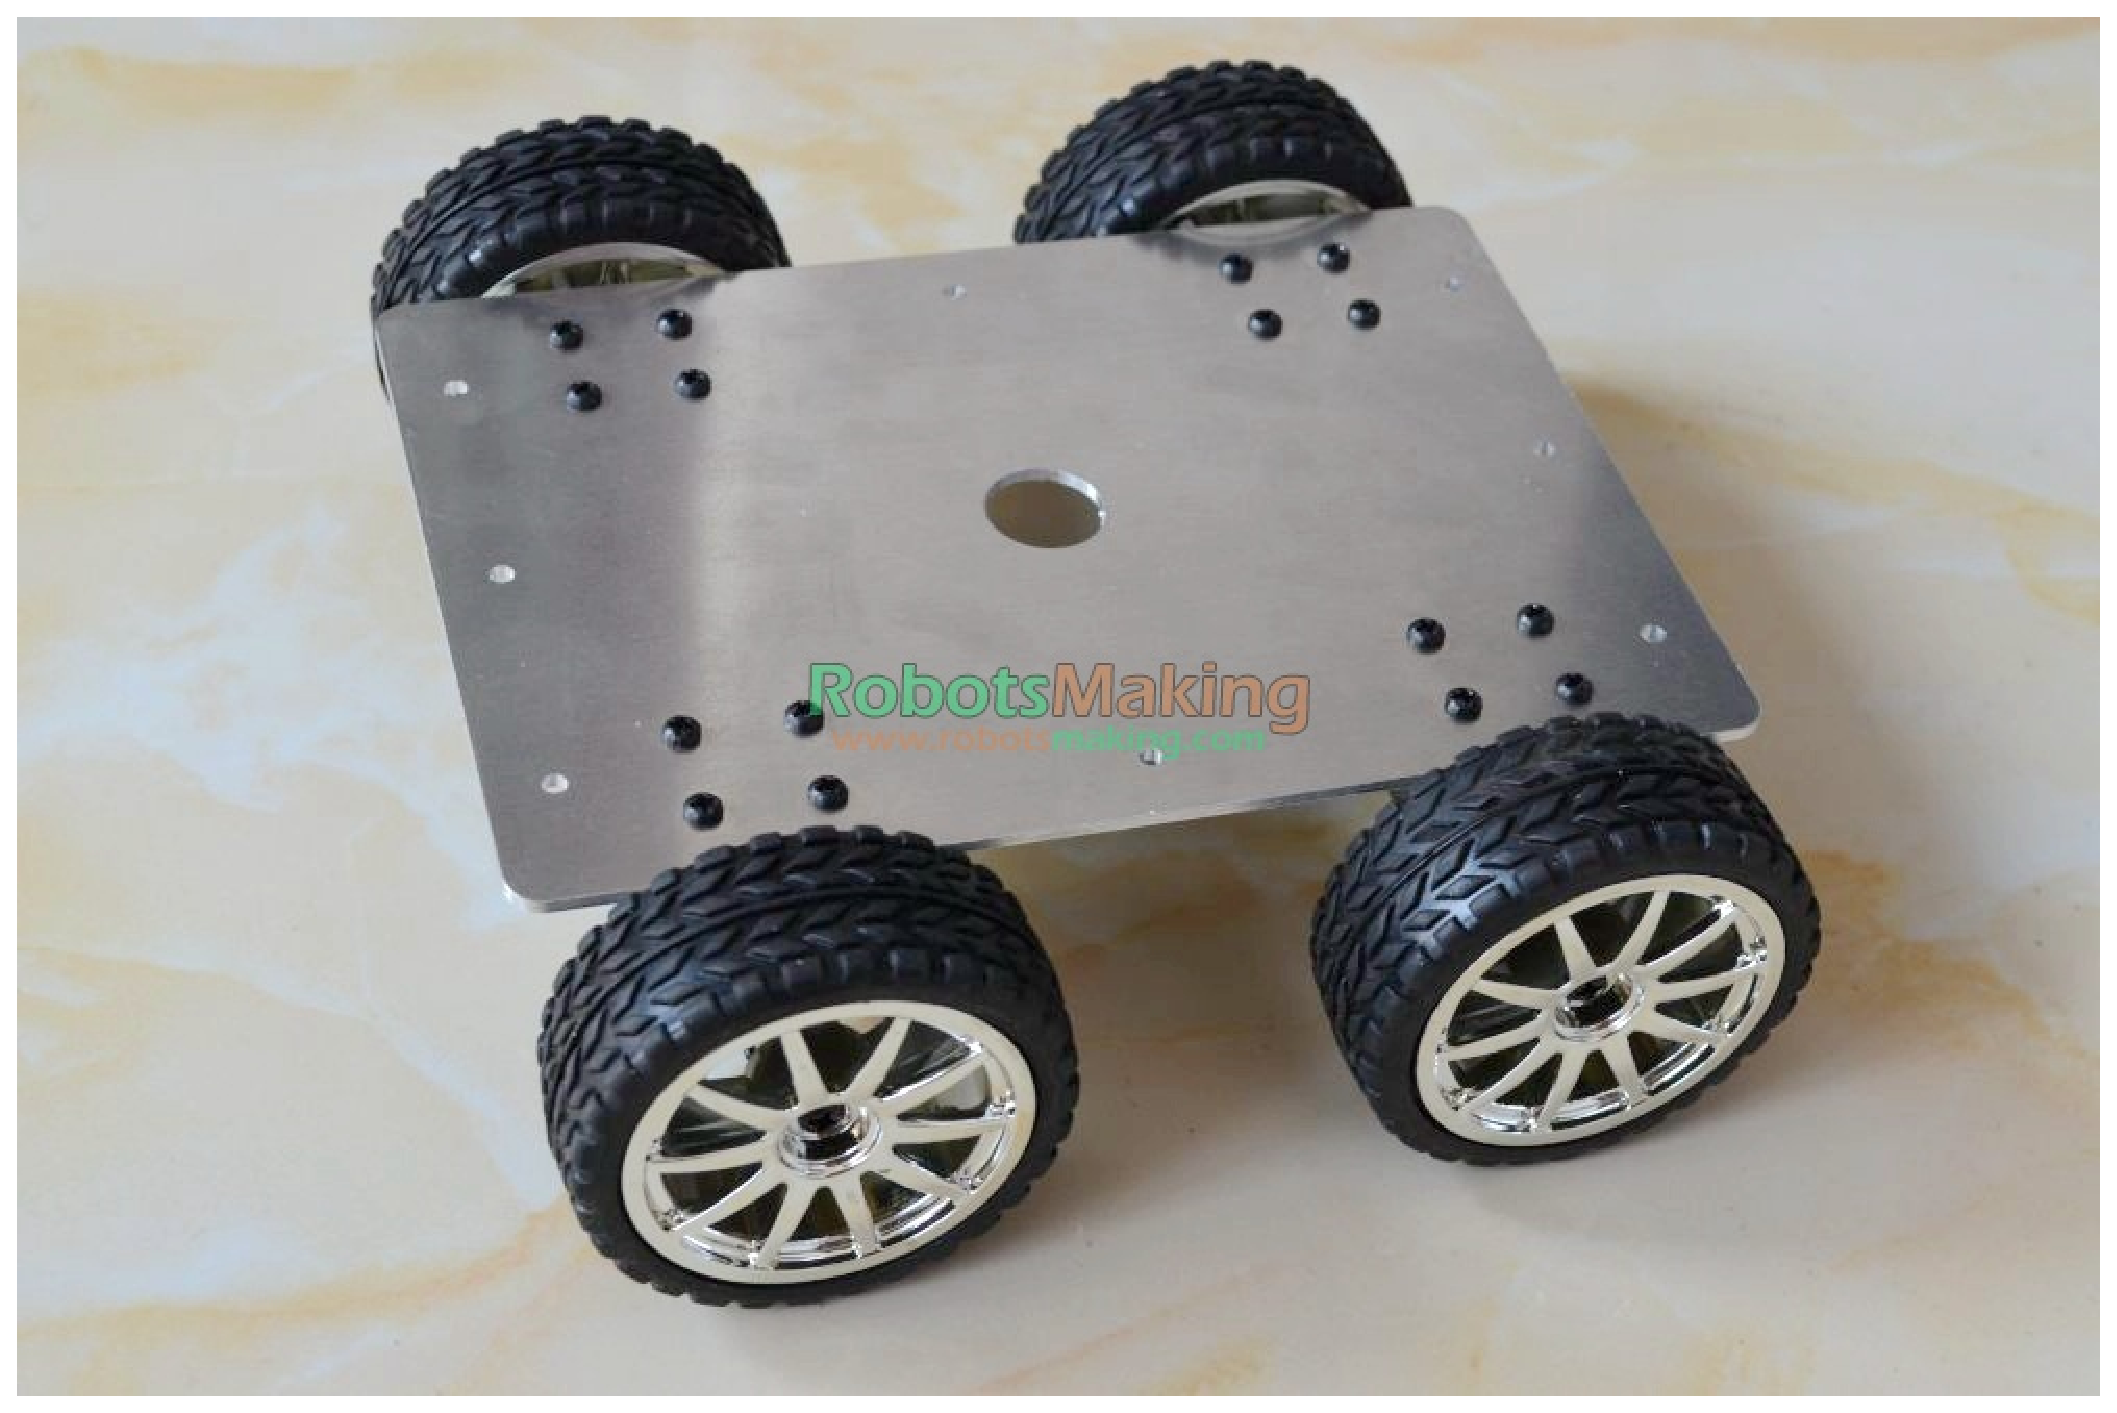
\includegraphics[width=2cm]{figuras/chassi_aluminio.eps} & \href{https://pt.aliexpress.com/store/product/New-25-aluminum-alloy-tracking-robot-tank-chassi-car-4WD-metal-tank-car-chassis-for-DIY/421824_32294898374.html}{pt.aliexpress.com}\\\hline
  \end{tabular}
  \end{center}
  \end{table}

  \begin{table}[!htbp]
  \begin{center}
  \caption{Eixo}
  \begin{tabular}{|p{2cm}|p{3cm}|p{2cm}|p{4cm}|}
  \hline
  \textbf{Eixo} & \textbf{Material} & \textbf{Imagem} & \textbf{Link}\\\hline\hline
  Tipo 1 & Aço inox & 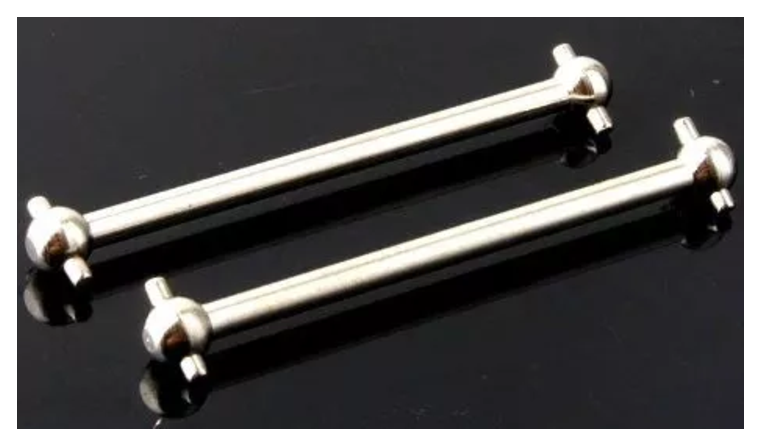
\includegraphics[width=2cm]{figuras/eixo_inox.eps} & \href{http://produto.mercadolivre.com.br/MLB-681527051-par-de-eixo-dogbone-84-mm-06061-redcat-himoto-exceed-hsp-_JM}{mercadolivre.com.br}\\\hline
  Tipo 2 & Aluminio  & 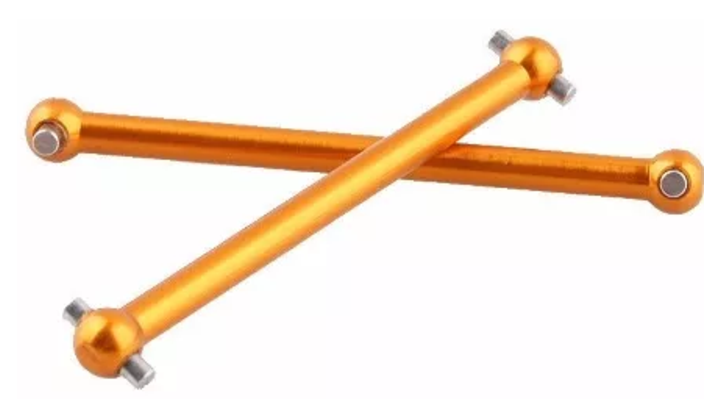
\includegraphics[width=2cm]{figuras/eixo_aluminio.eps} & \href{http://produto.mercadolivre.com.br/MLB-700430643-eixos-dogbones-em-aluminio-mastadon-spino-himoto-23608-par-_JM}{mercadolivre.com.br}\\\hline
  \end{tabular}
  \end{center}
  \end{table}

    \begin{table}[!htbp]
    	\begin{center}
    		\caption{Carenagem}
    		\begin{tabular}{|p{3cm}|p{3cm}|p{2cm}|p{4cm}|}
    			\hline
    			\textbf{Carenagem} & \textbf{Material} & \textbf{Imagem} & \textbf{Link}\\\hline\hline
    			Tipo 1 & Fibra de vidro & 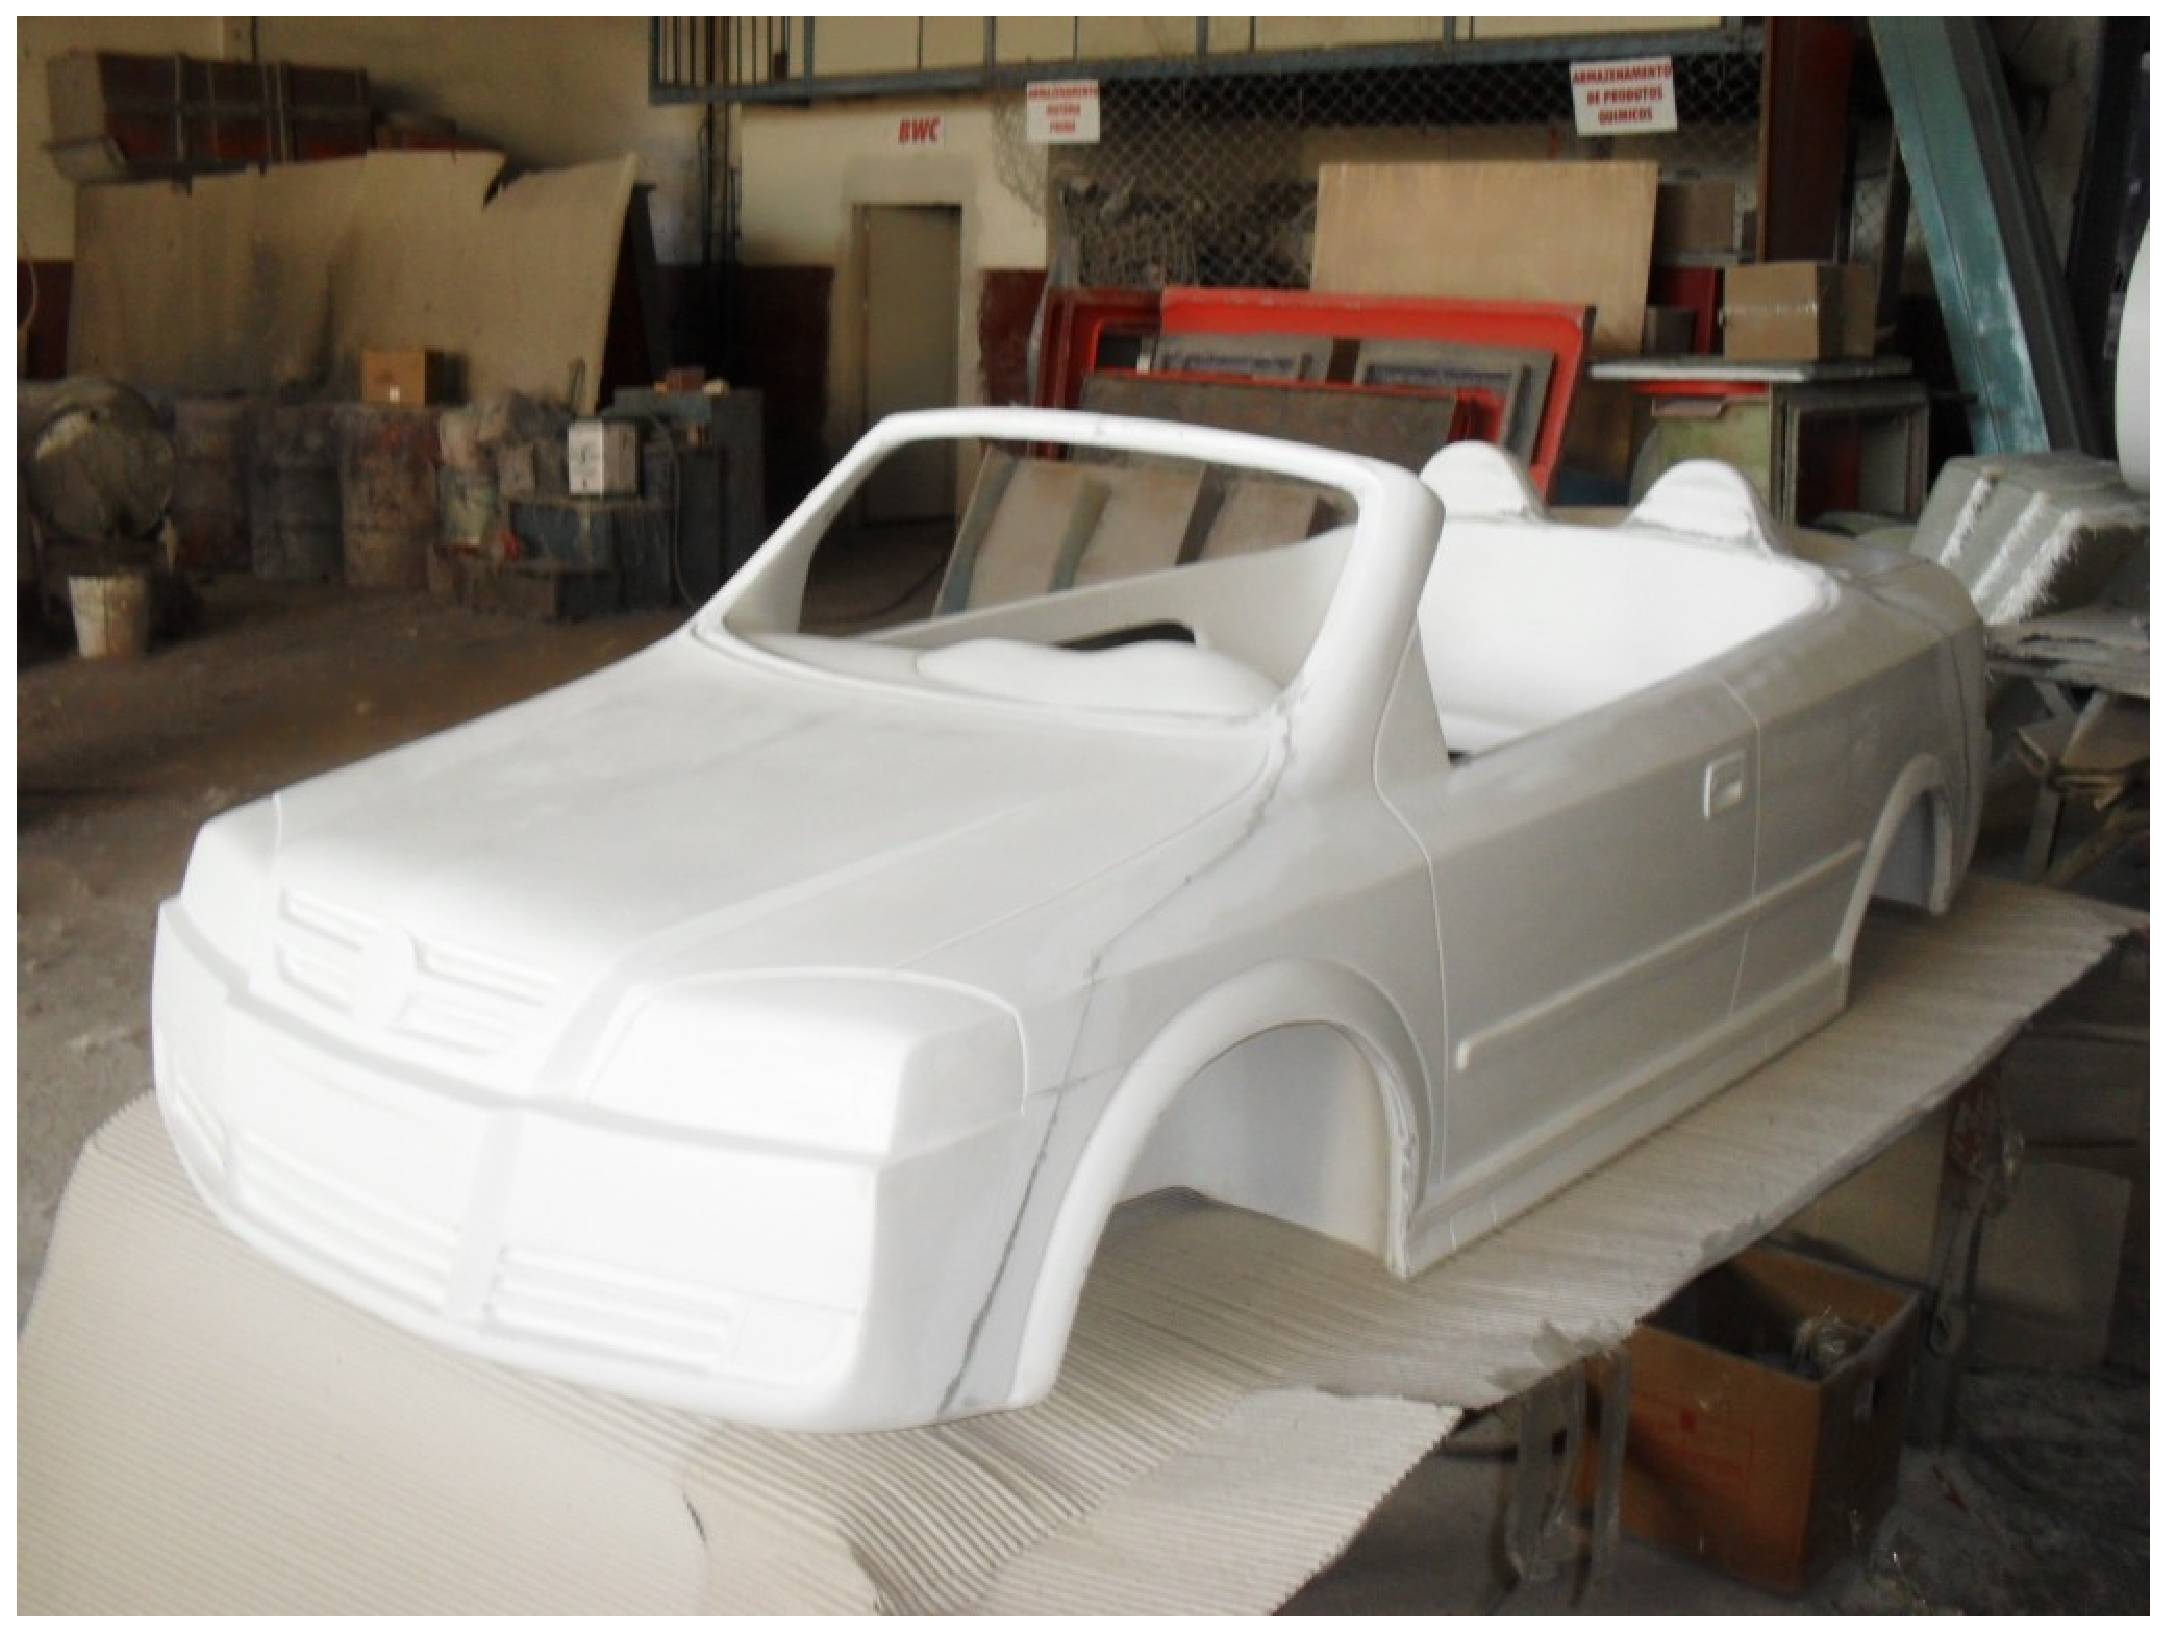
\includegraphics[width=2cm]{figuras/carenagem_fibra.eps} & \href{http://produto.mercadolivre.com.br/MLB-712761072-kit-resina-500g-manta-fibra-de-vidro-300g-10g-catalizador-_JM}{mercadolivre.com.br}\\\hline
    			Tipo 2 & Plástico de fibra de carbono para impressora 3D & 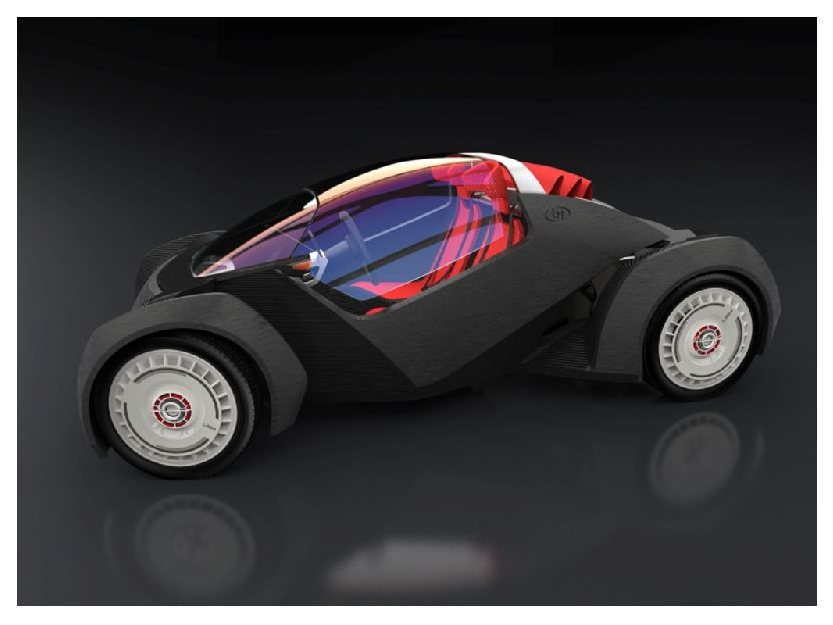
\includegraphics[width=2cm]{figuras/carenagem_plastico.eps} & \href{http://produto.mercadolivre.com.br/MLB-704169297-envelopamento-fibra-carbono-teto-ou-capo-1x122-_JM}{mercadolivre.com.br}\\\hline
    		\end{tabular}
    	\end{center}
    \end{table}

    \begin{table}[!htbp]
    	\begin{center}
    		\caption{Suspensão}
    		\begin{tabular}{|p{3cm}|p{3cm}|p{2cm}|p{4cm}|}
    			\hline
    			\textbf{Suspensão} & \textbf{Material} & \textbf{Imagem} & \textbf{Link}\\\hline\hline
    			Tipo 1 & Aluminio & 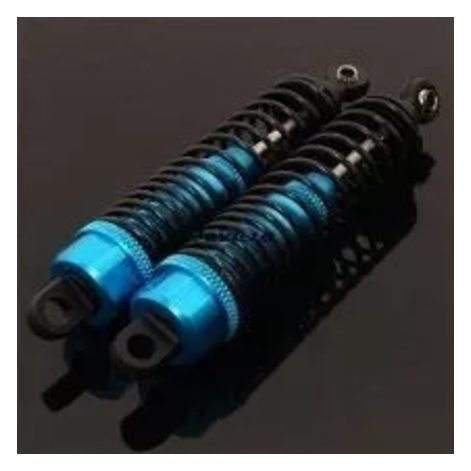
\includegraphics[width=2cm]{figuras/suspensao_aluminio_1.eps} & \href{http://produto.mercadolivre.com.br/MLB-689668697-par-amortecedor-aluminio-hsp-106004-06038-06062-rc-110-97mm-_JM}{mercadolivre.com.br}\\\hline
    			Tipo 2 & Aluminio & 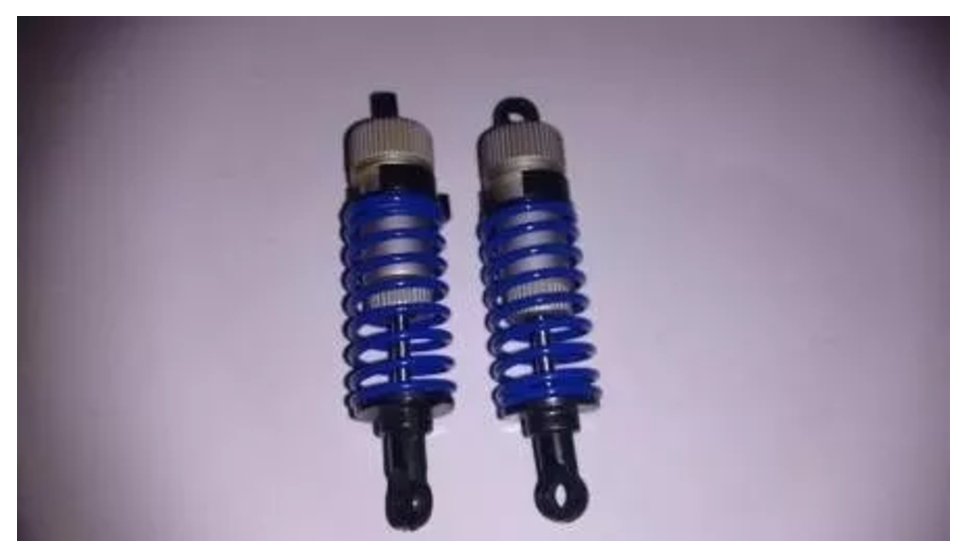
\includegraphics[width=2cm]{figuras/suspensao_aluminio_2.eps} & \href{http://produto.mercadolivre.com.br/MLB-722851070-par-de-amortecedor-75mm-para-automodelo-110-_JM}{mercadolivre.com.br}\\\hline
    		\end{tabular}
    	\end{center}
    \end{table}

    \newpage

  Ao comparar as características de cada material descrito acima, podemos chegar a conclusão que os melhores materiais que
  serão usados para a produção do veículo são:

  \begin{itemize}
    \item Roda + Pneu: a roda do tipo “off road”, pois a mesma é feita de material resistente e próprio para locomoção em estradas do tipo de terra. Já a roda de MBS possui o pneu de material inflável, logo o pneu pode furar durante o trajeto.
    \item Chassi: o alumínio é um material resistente à corrosão, durável, leve e fácil de trabalhar, já o chassi de aço, além de ser mais caro, é mais pesado e não é moldado facilmente. Dessa forma será utilizado o alumínio.
    \item Eixo: o aço inox para este caso, se encaixa melhor, pois possui maior dureza do que seu comparativo disponível.
    \item Carenagem: a fibra de vidro é um dos materiais mais usados para esse tipo de aplicação, porque é de baixo custo e muito fácil de trabalhar. Já o plástico de fibra de carbono, tem um custo maior, precisa de uma impressora 3D para imprimir a peça e de um projeto feito em um software compatível com a  impressora. Ou seja, o plástico de carbono demanda custo e tempo para fabricar uma peça.
  \end{itemize}


  \subsection{Sistema de Alimentação}

  \begin{itemize}
    \item Motores


    Para o projeto, os motores precisam apresentar um torque elevado e robustez
    devido ao ambiente em que será submetido, porém, não justifica o emprego de
    motores de precisão, como são os motores de passo. Portanto, a partir da
    análise das características dos motores existentes e considerando a satisfação
    dos requisitos do projeto, custos limitados e o tempo hábil para a construção
    e integração do produto em questão, os motores para tração escolhidos foram
    motores de corrente contínua.

    Sendo assim, determinou-se o uso de dois desses motores para cada roda
    traseira, com transmissões independentes, sendo essas responsáveis pelo torque
    do veículo. Essa escolha é justificada pela possibilidade de um terreno
    arenoso, altamente úmido, com imperfeições e desníveis. A utilização destes
    dois motores garante que não haja atolamento e que o produto possa se locomover sem
    maiores dificuldades.

    Para o dimensionamento dos motores de tração, foi necessário calcular a
    potência que o veículo demandará para seu deslocamento. Essa potência foi
    encontrada a partir da formulação:

      INSERIR FÓRMULA

    Onde  é o torque e  é a rotação em rpm. Sendo que o torque necessário foi calculado com base na formulação:

      INSERIR  OUTRA FÓRMULA

    Sendo  o número de peças acopladas ao eixo do motor,  o momento de inércia de cada peça em questão e  a área das mesmas peças.

    Tendo como parâmetros iniciais, massa do veículo de 16 kg e velocidade de deslocamento máxima de 2,7 m/s, foi possível obter aproximadamente 7,5 N.m de torque e 50W de potência. Para atender a essa demanda, optou-se por utilizar dois motores, um para cada lado, modelo Mabuchi GD – 558RC/LC 12 V. O qual possui 38 W e um torque máximo de 9,3 N.m.

Com o intuito de controlar a direção do veículo, o servomotor de direção 1/10 e 1/8 HPI foi selecionado para orientar as rodas da frente, visto que o mesmo deverá realizar manobras de até 180 graus ao final de cada fileira de morangos, contornando para a próxima. Um motor de passo também poderia satisfazer essa aplicação, porém o custo elevado e a satisfatória associação do servomotor com sensores cumprem os requisitos no projeto.

Para atender as demandas técnicas do projeto, o servomotor precisará ter torque elevado, para tanto foi o escolhido o servo HD LF-20mg 20KG, o qual possui torque máximo de 20 kg-cm.

    \item Bateria

    Algumas especificações devem ser observadas na seleção uma bateria, as mais importantes são a corrente e a
    tensão \cite{MAGALHAES}.

    Os cálculos de autonomia para as baterias não são triviais, necessitam de muitos parâmetros. Na literatura não
    há uma formulação exata para calcular esses valores. Portanto, são usadas diversas aproximações e parâmetros mais
    relevantes são determinados \cite{MEGGLIAR}.

    Três parâmetros principais que são apresentados: curva de descarga, a capacidade da bateria e a capacidade de
    descarga \cite{MEGGLIAR}.

    A curva de descarga representa o decaimento da tensão ao longo do consumo da capacidade nominal. O segundo parâmetro
    é a capacidade da bateria, o qual quantifica o tempo para que ocorra uma descarga total. Sua medida usual é Ah
    (Ampère x hora) \cite{MEGGLIAR}.

    A capacidade de descarga é quanto a bateria consegue fornecer sem que ocorra um superaquecimento, que poderia
    causar danos imensos a todo o projeto. Ela vem representada nas especificações pela letra C \cite{MEGGLIAR}.

    Alguns tipos de baterias poderiam ser selecionados para o projeto. A Bateria Íon- Lítio é o mais utilizado atualmente
    no mercado para aplicações em aparelhos eletrônicos, seu funcionamento consiste no uso de íons lítio presentes no
    eletrólito na forma sais dissolvidos em solventes não aquosos. Suas principais características são baixas taxas de auto
    descarga, longos ciclos de vida e segurança no manuseio \cite{castillo2002advances}.

    Em segundo, a bateria de polímero de lítio possui seus eletrólitos contidos em um polímero, diferentemente das baterias
    de íon-lítio, em que os eletrólitos estão contidos em solventes. As baterias de polímero de lítio são baterias de tecnologia
    ultrafinas. Isso é possível devido a sua maior densidade de energia quando comparada com as baterias de íon- lítio.

    Por fim, as baterias de chumbo-ácido são baterias comumente utilizadas em arranques e iluminação para automóveis,
    sistemas de tração para veículos e máquinas elétricas, além de serem utilizadas como fontes alternativas em nobreaks.
    Sua composição é chumbo, que está presente na forma sólida e ácido sulfúrico, em concentração que varia de 27\% a 37\%
    \cite{pulsada2005juliano}. Se apresentam em dois formatos: seladas e não seladas, sendo que nesta segunda existe a necessidade de
    reposição de água. São baterias recarregáveis, pesadas, têm vida útil de até quatro anos e possuem custo-benefício satisfatório.

    Para o correto dimensionamento, levantou-se o consumo dos componentes do veículo, como pode ser visto na tabela \ref{tabeladimensionamento}.

     \begin{table}[!htbp]
     \centering
     \caption{Tabela de dimensionamento de consumo dos componentes}
     \label{tabeladimensionamento}
     \begin{tabular}{|p{4cm}|p{4cm}|p{4cm}|}
     \hline
     Componente          & Corrente Máxima & Tensão Nominal \\\hline
     Arduino             & 2 A             & 5 - 20 V       \\\hline
     Raspberry           & 2 A             & 5 V            \\\hline
     Driver              & 4 A cada        & 4-35 V         \\\hline
     Motor DC Tração     & 2 A cada        & 12 V           \\\hline
     Motor DC Perfuração & 2 A cada        & 12 V           \\\hline
     Servomotor          & 2 A             & 6 V            \\\hline
     \end{tabular}
     \end{table}

     Um ponto importante é observar que como os motores estarão conectados aos seus respectivos drivers de controle as
     correntes máximas são limitadas por eles. Como serão dois drivers de controle, a corrente máxima necessária será de
     14 A. Portanto, para 1 hora de operação em carga máxima, será necessário uma bateria de 14 Ah. Optou-se pelo modelo Get
     Power gp12-14, ela possui 12 V e 14 Ah.

     Para recarregar a bateria foi cogitado a utilização de um painel solar. Porém, a placa solar possui dimensões maiores
     que a estrutura do carro e um baixo ganho energético, em torno de apenas 3\%, o que não viabiliza a sua aplicação nesse
     projeto.

     \item Circuito Elétrico

     O diagrama unifilar apresentado na figura \ref{diagramaunifilar} representa as ligações a serem realizadas entre os componentes que serão utilizados.
     Após a bateria, será colocado um disjuntor monopolar (no ponto D) de 17,5 A de corrente alternada. Apesar de não ser de
     corrente contínua, ele satisfaz os requisitos de operação. Para o Arduino e para a Raspberry determinou-se dois fusíveis
     (F1 e F2) de 3 A.

     \begin{figure}[!htbp]
     \begin{center}
     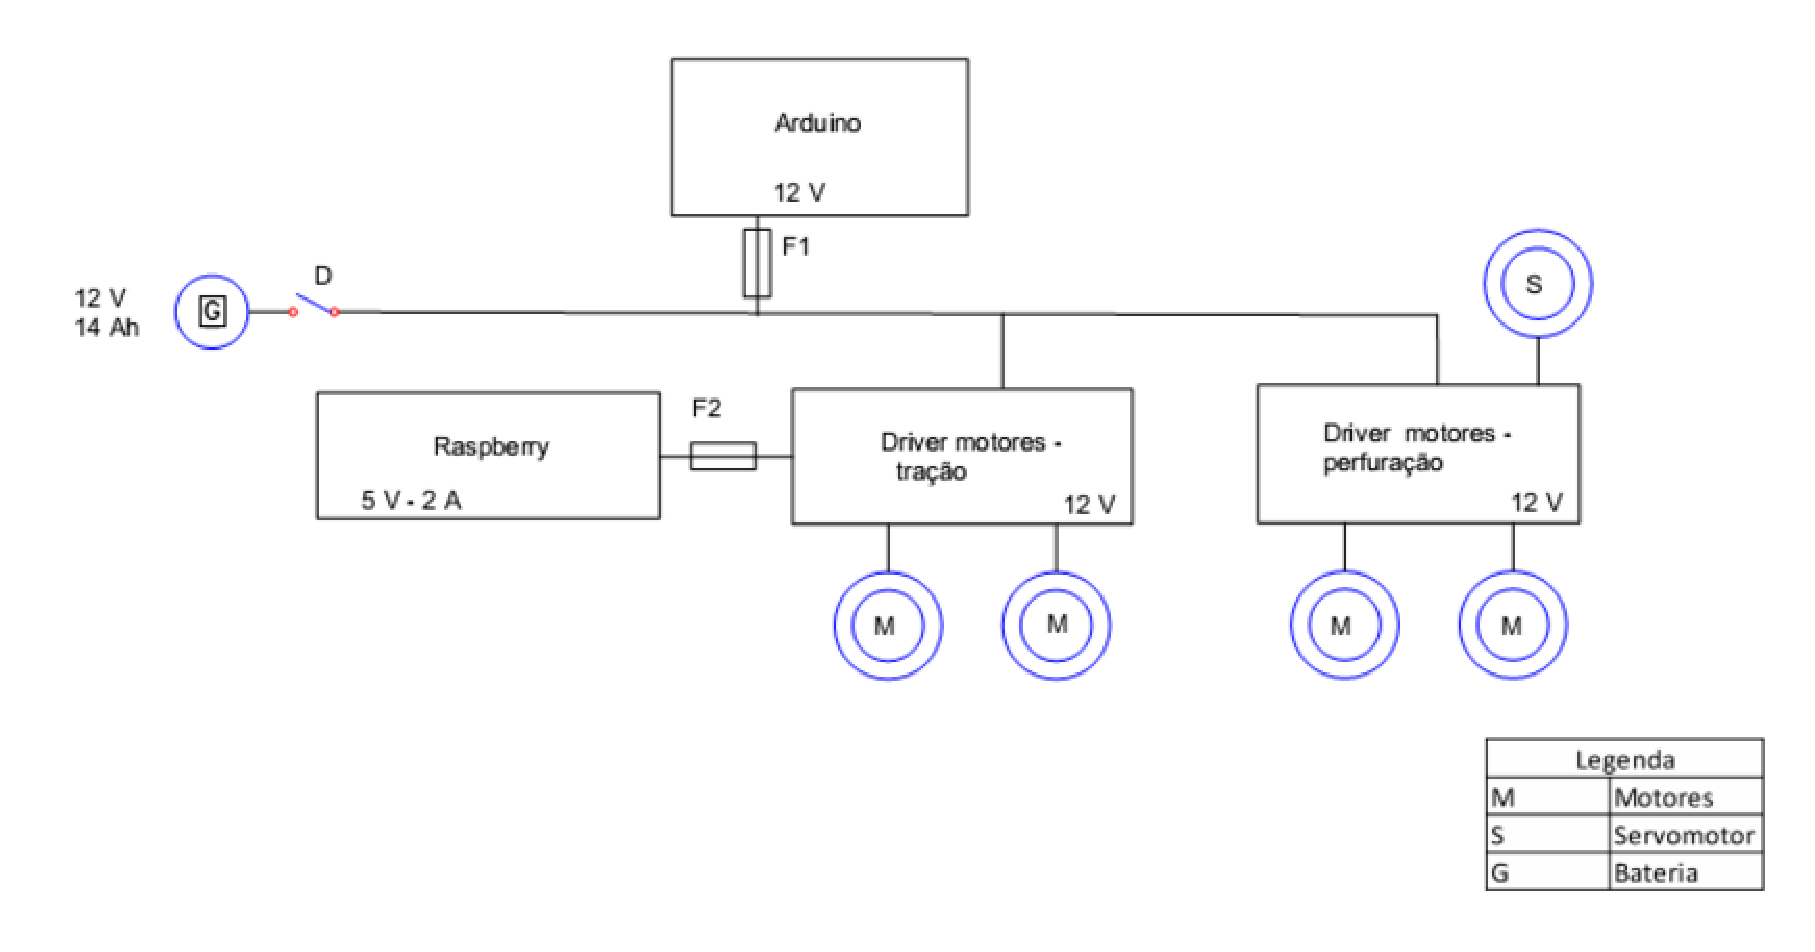
\includegraphics[keepaspectratio=true,scale=0.5]{figuras/diagramaunifilar.eps}
     \caption{\label{diagramaunifilar}Diagrama Unifilar dos Componentes}
     \end{center}
     \end{figure}

  \end{itemize}
